\documentclass[superscriptaddress,reprint,amsmath,amssymb,aps]{revtex4-1}
%\documentclass[english,prl,reprint,amsmath,amssymb,aps,superscriptaddress]{revtex4}
%\usepackage{amsmath}
%\usepackage{amssymb}
\usepackage{graphicx}% Include figure files
%\usepackage{babel}
\usepackage{dcolumn}% Align table columns on decimal point
\usepackage{bm}% bold math
\usepackage{supertabular}

\begin{document}

\pagenumbering{gobble}

\begin{figure*}
\begin{picture}(0,140)
\put(-240,130){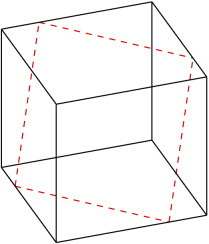
\includegraphics[width=1.6in,angle=-90]{fig1a}}
\put( -90,  0){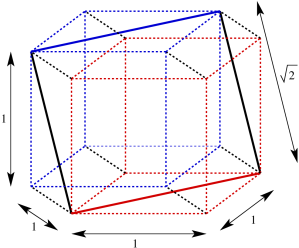
\includegraphics[width=2.3in,angle=  0]{fig1b}}
\put( 100,  5){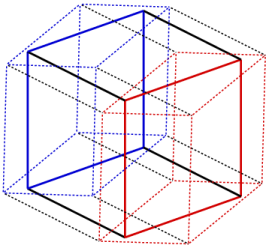
\includegraphics[width=2.0in,angle=  0]{fig1c}}
\end{picture}
\caption{\label{fig:fig1}
(a) Nieuwland's optimal solution to Rupert's original problem where the
    square's vertices divide the cube's edges in the length ratio of 1:3.
(b) The maximal square within a tesseract.
(c) The maximal cube within a tesseract.
}
\label{fig1}
\end{figure*}

\begin{figure*}
\begin{picture}(0,170)
\put(-280,170){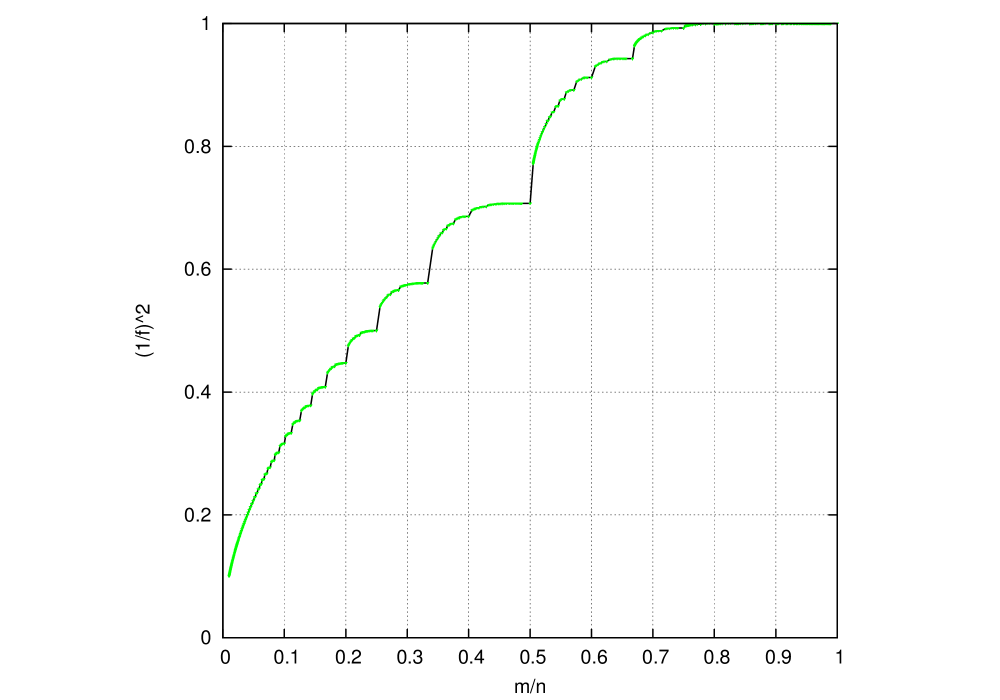
\includegraphics[width=2.5in,angle=-90]{fig3a}}
\put( -20,170){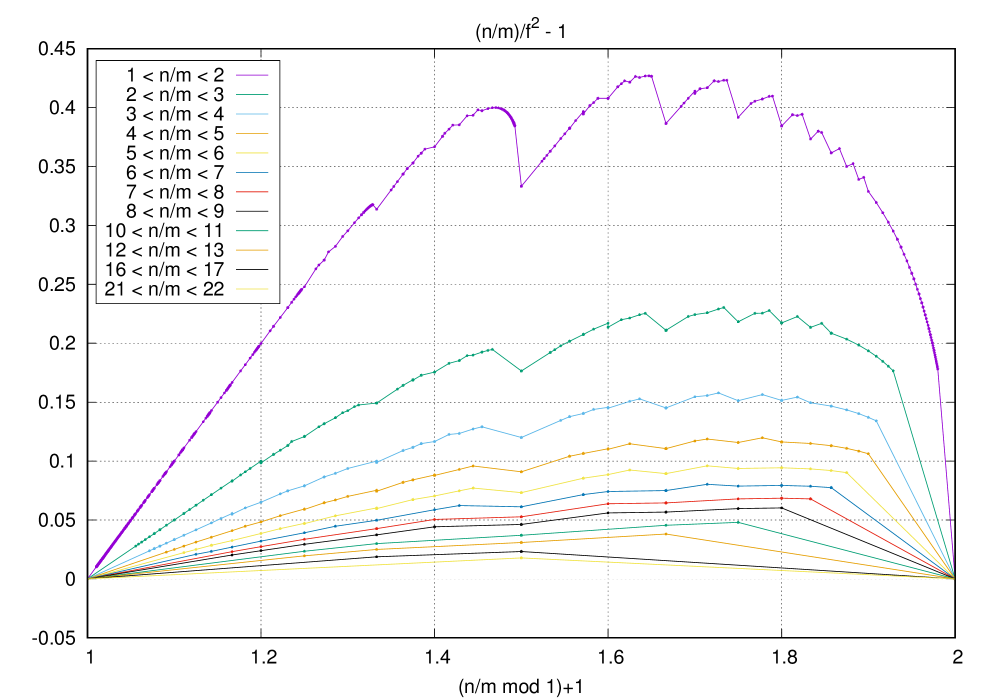
\includegraphics[width=2.5in,angle=-90]{fig3b}}
\end{picture}
\caption{\label{fig:fig3}
(a) Inverse square of the edge length as a function of $m/n$.
(b) $1/f^2 - n/m$ versus $(n/m~\text{mod}~1)+1$.
}
\label{fractalplots}
\end{figure*} 

\begin{figure*}
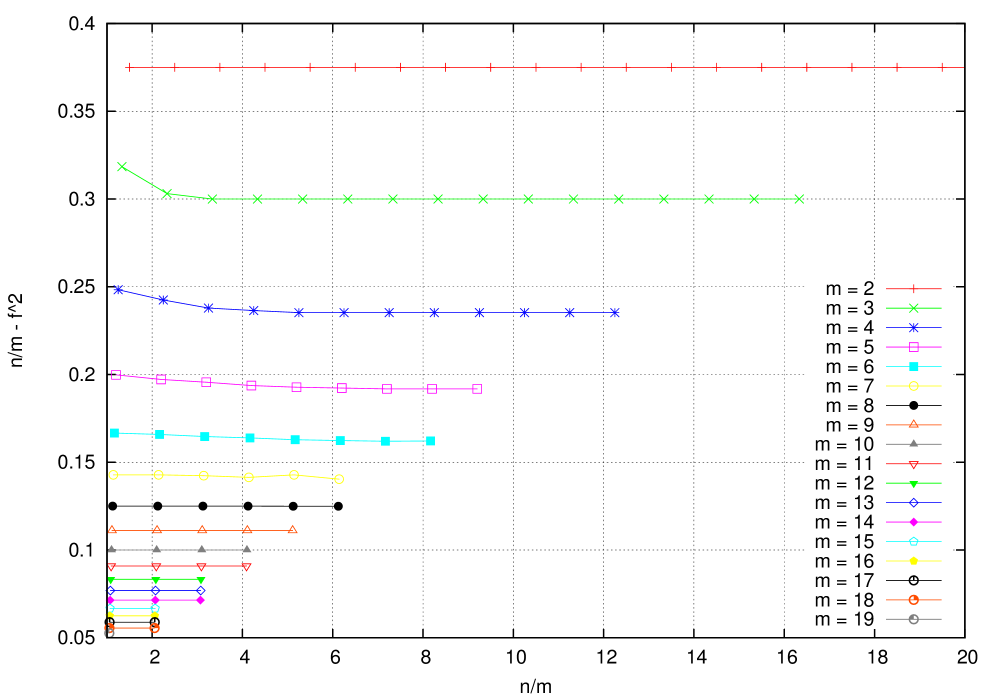
\includegraphics[angle=-90,width=4.5in]{fig4}
\vspace{-0.1in}
\caption{\label{fig:fig4} Energies of families of solutions as a function of $n/m$.}
\label{families}
\end{figure*} 

\end{document}
